\documentclass[a4paper, 11pt]{article}

\usepackage[a4paper,margin=1in]{geometry}
\usepackage[french]{babel}
\usepackage[utf8]{inputenc}
\usepackage[T1]{fontenc}
\usepackage{lmodern}
\usepackage{listings}
\usepackage{graphicx}
\usepackage{amsmath}
\usepackage{framed}
\usepackage{amsfonts}
\usepackage{caption}
\usepackage{subcaption}
\usepackage{listings}
\usepackage{tabularx}
\usepackage{color}
\usepackage[dvipsnames]{xcolor}
\usepackage{fancyhdr}
\usepackage{lastpage}
\usepackage{tikz}

\usetikzlibrary{decorations.pathreplacing, matrix}

\graphicspath{{../imgs/}}


\definecolor{morange}{RGB}{237,106,90}
\definecolor{mgreen}{RGB}{63,127,95}
\definecolor{mpurple}{RGB}{127,0,85}

\lstset{
  basicstyle=\small\ttfamily, % Global Code Style
  captionpos=b, % Position of the Caption (t for top, b for bottom)
  extendedchars=true, % Allows 256 instead of 128 ASCII characters
  tabsize=2, % number of spaces indented when discovering a tab
  columns=fixed, % make all characters equal width
  keepspaces=true, % does not ignore spaces to fit width, convert tabs to spaces
  showstringspaces=false, % lets spaces in strings appear as real spaces
  breaklines=true, % wrap lines if they don't fit
  frame=trbl, % draw a frame at the top, right, left and bottom of the listing
  frameround=tttt, % make the frame round at all four corners
  framesep=4pt, % quarter circle size of the round corners
  numbers=left, % show line numbers at the left
  numberstyle=\tiny\ttfamily, % style of the line numbers
  commentstyle=\color{mgreen}, % style of comments
  keywordstyle=\color{mpurple}, % style of keywords
  stringstyle=\color{morange}, % style of strings
}

% TAILLE DES PAGES (A4 serré)

\setlength{\parindent}{0pt}
\setlength{\parskip}{1em}
%% \setlength{\textwidth}{17cm}
%% \setlength{\textheight}{24cm}
%% \setlength{\oddsidemargin}{-.7cm}
%% \setlength{\evensidemargin}{-.7cm}
%% \setlength{\topmargin}{-.5in}


\pagestyle{fancy}
\renewcommand{\headrulewidth}{0pt}
\renewcommand{\footrulewidth}{0.6pt}% default is 0pt
\lhead{}
\rhead{}
\lfoot{Page \thepage\ of \pageref{LastPage}}
\rfoot{Rémi Lespinet}
\cfoot{}
\cfoot{}



\newcounter{cquestion}[subsection]
\renewcommand{\thecquestion}{\arabic{cquestion}}
\newenvironment{question}
{\par \vspace{0.5em} \noindent \stepcounter{cquestion} \hspace{-1em}
 $\bullet$ \underline{Q\thecquestion :}}
{}

\newenvironment{note}
{\begin{framed} \textbf{Note : }}
{\end{framed}}


% Commandes de mise en page
\newcommand{\file}[1]{\emph{#1}}
\newcommand{\name}[1]{\emph{#1}}
\newcommand{\Fig}[1]{Fig \ref{#1} p. \pageref{#1}}
\newcommand{\Figure}[1]{Figure \ref{#1} p. \pageref{#1}}
\newcommand{\Tab}[1]{Tab \ref{#1} p. \pageref{#1}}
\newcommand{\Table}[1]{Table \ref{#1} p. \pageref{#1}}
\newcommand{\itemi}{\item[$\bullet$]}
% Commandes color
\newcommand{\colgood}[1]{\color{ForestGreen} #1}
\newcommand{\colbad}[1]{\color{BrickRed} #1}


% Commandes de maths
\newcommand{\function}[3]{#1 : #2 \to #3}
\newcommand{\intn}[2]{\left\{ #1 \dots #2 \right\}}
\newcommand{\intr}[2]{\left[ #1 ; #2 \right]}
\newcommand{\intro}[2]{\left] #1 ; #2 \right[}
\newcommand{\dotp}[2]{\langle #1, #2 \rangle}
\newcommand{\logn}[1]{\ln\left( #1\right)}
%% \newcommand{\det}[1]{\left| #1 \right|}
\newcommand{\pd}[2]{\frac{\partial #1}{\partial #2}}
\newcommand{\norm}[1]{\|#1\|}
\newcommand{\set}[2]{\left\{ #1 \hspace{.5em} ; \hspace{.5em}#2 \right\}}
\newcommand{\tr}[1]{Tr\left( #1 \right)}
\newcommand{\pcond}[2]{p(#1 \hspace{-.2em}\mid\hspace{-.2em} #2)}

\newcommand{\grad}[1]{\nabla{#1}}
\newcommand{\jac}[1]{\text{D}#1}


\newcommand{\iid}{i.i.d }
\newcommand{\wrt}{w.r.t }

% Commandes informatique
\newcommand{\pfun}[1]{{\textbf{\texttt{#1}}}}

\newcommand{\ipart}[1]{\vspace{0.5em}\textbf{#1}\vspace{0.5em}}

\newcolumntype{C}[1]{>{\centering\arraybackslash$}p{#1}<{$}}

\pagenumbering{arabic}

\title{\textsc{Convex optimization - MVA 2017/2018 \\ \emph{Homework 3}} }
\author{Rémi Lespinet}
\date{}

\begin{document}

\maketitle
\thispagestyle{fancy}

\section{Interior Points Method}

If $\function{f}{\mathbb{R}^n}{\mathbb{R}}$ and
$\function{g}{\mathbb{R}^p}{\mathbb{R}^n}$, then
\begin{equation*}
  \nabla{(f \circ g)}(x) = \jac{g(x)}^T \nabla{f}(g(x))
\end{equation*}
and if
$\function{f}{\mathbb{R}^n}{\mathbb{R}^q}$ and
$\function{g}{\mathbb{R}^p}{\mathbb{R}^n}$, then
\begin{equation*}
  \jac{(f \circ g)}(x) = \jac{f}(g(x)) \jac{g(x)}
\end{equation*}

\begin{question}
   We have
  \begin{equation*}
    \nabla{\phi}(x) = Q x + p
  \end{equation*}
  and
  \begin{equation*}
    \pd{B}{x_j}(x) = - \dfrac{1}{x_j}
  \end{equation*}
  Let $\Psi$ be the function
  \begin{equation*}
    \begin{array}{lccc}
      \Psi \colon & \mathbb{R}^N &\to& \mathbb{R}^N \\
                        & \left(x_1, \dots, x_N\right) &\mapsto& \left(\dfrac{1}{x_1}, \dots, \dfrac{1}{x_N}\right)
    \end{array}
  \end{equation*}
  We can write
  \begin{equation*}
    \nabla{B}(x) = - \Psi(x)
  \end{equation*}
  If we note $f$ the function
  \begin{equation*}
    \begin{array}{lccc}
    f \colon & \mathbb{R}^d &\to& \mathbb{R}^N\\
    & x &\mapsto& b - A x
    \end{array}
  \end{equation*}
  It's jacobian is given by
  \begin{equation*}
    \jac{f}(x) = -A
  \end{equation*}
  Thus
  \begin{framed}
    \begin{equation*}
      \nabla{\phi_t}(x) = t (Q x + p) + A^T \Psi(b - A x)
    \end{equation*}
  \end{framed}
\end{question}

\begin{question}
  Obviously,
  \begin{equation*}
    \nabla^2{B}(x) = \jac{\Psi}(x) = \text{diag}\left[ -\dfrac{1}{x_1^2}, \dots, -\dfrac{1}{x_d^2}\right]
  \end{equation*}
  Let $\Psi$ be the function
  \begin{equation*}
    \begin{array}{lccc}
      \Theta \colon & \mathbb{R}^N &\to& \mathbb{R}^N\\
                    & \left(x_1, \dots, x_N\right) &\mapsto& \text{diag}\left(\dfrac{1}{x_1^2}, \dots, \dfrac{1}{x_N^2}\right)
    \end{array}
  \end{equation*}
  We can rewrite the precedent expression as
  \begin{equation*}
    \nabla^2{B}(x) = \jac{\Psi}(x) = - \Theta(x)
  \end{equation*}

  Then
  \begin{equation*}
    \jac{(\Psi \circ f)}(x) = \Theta{(b - A x)} A
  \end{equation*}
  Hence,
  \begin{framed}
    \begin{equation*}
      \nabla^2{\phi_t}(x) = t Q +  A^T \Theta{(b - A x)} A
    \end{equation*}
  \end{framed}

\end{question}

\section{Support Vector Machine Problem}

\begin{question}
  For the primal problem (SVM-P), we can take
  \begin{equation*}
    z = (1 + \epsilon, \dots, 1 + \epsilon)
  \end{equation*}
  and
  \begin{equation*}
    w = (0, \dots, 0)
  \end{equation*}

  For the dual problem (SVM-D), we can take
  \begin{equation*}
    \lambda = (\dfrac{1}{2 \tau n}, \dots, \dfrac{1}{2 \tau n})
  \end{equation*}

\end{question}


\begin{question}

  For the primal, we obtain
  \begin{equation*}
    \begin{array}{lll}
      X = \left[
      \begin{array}{c}
        w_1 \\
        \vdots \\
        w_d \\
        z_1 \\
        \vdots \\
        z_N
      \end{array}
      \right]
      &
        P = \left[
        \begin{array}{c}
          0 \\
          \vdots \\
          0 \\
          \frac{1}{\tau n} \\
          \vdots \\
          \frac{1}{\tau n}
        \end{array}
      \right]
      &
    Q =
    \begin{tikzpicture}[baseline=(current bounding box.center),
      decoration=brace,
      large/.style={font=\large}]
      \matrix (M)[matrix of math nodes, nodes in empty cells,
      left delimiter={[}, right delimiter={]},
      column sep={1.2em,between origins},
      row sep={1.2em,between origins}
      ]{ 1       &    &   &   &   &   & & & \\
        & \ddots &    &   &   &   &   & & \\
       &       &  1 &   &   &   &   & & \\
        &        &    &   &   &   &   & & \\
        &        &    &   &   &   &   & & \\
        &        &    &   &   &   &   & & \\
        &        &    &   &   &   &   & & \\
        &        &    &   &   &   &   & & \\
        &        &    &   &   &   &   & & \\
      };
      \draw(M-1-4.north)--(M-9-4.south);
      \draw(M-4-1.west)--(M-4-9.east);
      \node[large] at (M-2-7){$0$};
      \node[large] at (M-7-2){$0$};
      \node[large] at (M-7-7){$0$};
      \draw[decorate, transform canvas={yshift=0.8em}, thick] (M-1-1.mid west) -- node[above=2pt]{$d$}(M-1-3.mid east);
      \draw[decorate, transform canvas={yshift=0.8em}, thick] (M-1-5.mid west) -- node[above=2pt]{$n$}(M-1-9.mid east);
    \end{tikzpicture}
    \end{array}
  \end{equation*}

  and,
  \begin{equation*}
    \begin{array}{cc}
    A =
    \begin{tikzpicture}[baseline=(current bounding box.center),
      decoration=brace,
      large/.style={font=\large}]
      \matrix (M)[matrix of math nodes, nodes in empty cells,
      left delimiter={[}, right delimiter={]},
      column sep={1.2em,between origins},
      row sep={1.2em,between origins}
      ]{&  - y_1 x_1 & & & -1 &    &    &   & \\
        &  - y_2 x_2 & & &    & -1 &    &   & \\
        &  - y_3 x_3 & & &    &    & \ddots &   & \\
        &   \vdots   & & &    &    &    & -1&\\
        &  - y_N x_N & & &    &    &    &   & -1 \\
        & & & & &    &    &   & \\
        & & & & -1 &    &    &   & \\
        & & & &    & -1 &    &   & \\
        & & & &    &    & \ddots &   & \\
        & & & &    &    &    & -1&\\
        & & & &    &    &    &   & -1 \\
      };
      \draw(M-1-4.north)--(M-11-4.south);
      \draw(M-6-1.west)--(M-6-9.east);
      % \draw(M-4-1.mid)--(M-4-9.mid);
      \node[large, transform canvas={xshift=0.3em, yshift=0.6em}] at (M-9-2){$0$};
      % \node[large] at (M-7-2){$0$};
      % \node[large] at (M-7-7){$0$};
      \draw[decorate,transform canvas={yshift=0.8em},thick] (M-1-1.mid west) -- node[above=2pt]{$d$}(M-1-3.mid east);
      \draw[decorate,transform canvas={yshift=0.8em},thick] (M-1-5.mid west) -- node[above=2pt]{$n$}(M-1-9.mid east);
      % \draw[decorate,thick] (M-9-9.north) -- node[below=2pt]{$n$}(M-9-5.north);
    \end{tikzpicture}
    &
    B = \left[
      \begin{array}{c}
        -1 \\
        -1 \\
        \vdots \\
        -1 \\
        -1 \\
        0 \\
        0 \\
        \vdots \\
        0 \\
        0 \\
      \end{array}
      \right]
    \end{array}
  \end{equation*}

  For the dual, we notice that this is equivalent to
  \begin{equation*}
    \begin{aligned}
      % & \underset{\lambda}{\text{minimize}}
      & \text{minimize}
      & & \dfrac{1}{2} \norm{\sum_{i = 1}^N \lambda_i y_i x_i}_2^2 - \textbf{1}^T \lambda \\
      & \text{subject to}
      & & 0 \le \lambda \le \frac{1}{\tau n}\\
    \end{aligned}
  \end{equation*}
  Hence,
  \begin{equation*}
    \begin{array}{lll}
      X = \left[
      \begin{array}{c}
        \lambda_1 \\
        \lambda_2 \\
        \vdots \\
        \lambda_{N-1} \\
        \lambda_N \\
      \end{array}
      \right]
      &
        P = \left[
        \begin{array}{c}
        -1 \\
        -1 \\
        \vdots \\
        -1 \\
        -1 \\
        \end{array}
      \right]
      &
    \end{array}
  \end{equation*}

  we have $Q = S^T S$ with
  \begin{equation*}
    S =
    \begin{tikzpicture}[baseline=(current bounding box.center),
      decoration=brace,
      large/.style={font=\large}]
      \matrix (M)[matrix of math nodes, nodes in empty cells,
      left delimiter={[}, right delimiter={]},
      column sep={3.0em,between origins},
      row sep={1.2em,between origins}
      ]{& & & & \\
        & & & & \\
        y_1 x_1 & x_2 y_2 & x_3 y_3 & \hdots & x_N y_N\\
        & & & & \\
        & & & & \\
      };
      \draw[transform canvas={xshift=1.5em}](M-1-1.north)--(M-5-1.south);
      \draw[transform canvas={xshift=1.5em}](M-1-2.north)--(M-5-2.south);
      \draw[transform canvas={xshift=1.5em}](M-1-3.north)--(M-5-3.south);
      \draw[transform canvas={xshift=1.5em}](M-1-4.north)--(M-5-4.south);
      % \draw(M-4-1.mid)--(M-4-9.mid);
      % \node[large] at (M-2-7){$0$};
      % \node[large] at (M-7-2){$0$};
      % \node[large] at (M-7-7){$0$};
      % \draw[decorate, transform canvas={yshift=0.8em}, thick] (M-1-1.mid west) -- node[above=2pt]{$n$}(M-1-9.mid east);
    \end{tikzpicture}
  \end{equation*}
  Indeed,
  \begin{equation*}
    S \lambda = \sum_{i = 1}^N \lambda_i x_i y_i
  \end{equation*}


  and,
  \begin{equation*}
    \begin{array}{cc}
    A =
    \begin{tikzpicture}[baseline=(current bounding box.center),
      decoration=brace,
      large/.style={font=\large}]
      \matrix (M)[matrix of math nodes, nodes in empty cells,
      left delimiter={[}, right delimiter={]},
      column sep={1.8em,between origins},
      row sep={1.2em,between origins}
      ]{-1 &    &        &    &    \\
           & -1 &        &    &    \\
           &    & \ddots &    &    \\
           &    &        & -1 &    \\
           &    &        &    & -1 \\
           &    &        &    &    \\
         1 &    &        &    &    \\
           &  1 &        &    &    \\
           &    & \ddots &    &    \\
           &    &        &  1 &    \\
           &    &        &    &  1 \\
      };
      \draw(M-6-1.west)--(M-6-5.east);
      % \draw(M-4-1.mid)--(M-4-9.mid);
      % \node[large] at (M-2-7){$0$};
      % \node[large] at (M-7-2){$0$};
      % \node[large] at (M-7-7){$0$};
      \draw[decorate,transform canvas={xshift=0.3em, yshift=0.8em},thick] (M-1-1.mid west) -- node[above=2pt]{$n$}(M-1-5.mid east);
      \draw[decorate,transform canvas={xshift=2.2em},thick] (M-1-5.north) -- node[right=1pt]{$n$}(M-5-5.south);
      \draw[decorate,transform canvas={xshift=2.2em},thick] (M-7-5.north) -- node[right=1pt]{$n$}(M-11-5.south);
      % \draw[decorate,thick] (M-9-9.north) -- node[below=2pt]{$n$}(M-9-5.north);
    \end{tikzpicture}
    &\hspace{4em}
    B = \left[
      \begin{array}{c}
        0 \\
        0 \\
        \vdots \\
        0 \\
        0 \\
        \frac{1}{\tau n} \\
        \frac{1}{\tau n} \\
        \vdots \\
        \frac{1}{\tau n} \\
        \frac{1}{\tau n} \\
      \end{array}
      \right]
    \end{array}
  \end{equation*}

  TODO : we should exploit the structure

\end{question}

\begin{question}
  \ipart{Effect of $\tau$}

  The figure \ref{fig:iris-tau} shows the performance of the
  classifier on the Iris dataset (considering only the 2 classes
  \name{Iris-versicolor} and \name{Iris-virginica}) as a function of
  $\tau$. Each sample has a probability $p = 0.8$ (Bernoulli
  distribution) of being selected for the training, $mu = 10$,
  $tol = 0.01$. For the curve to be smoother, I ran the procedure $20$
  times and average the peformance ratio obtained on these $20$
  iterations.

  \begin{figure}[h]
    \centering
    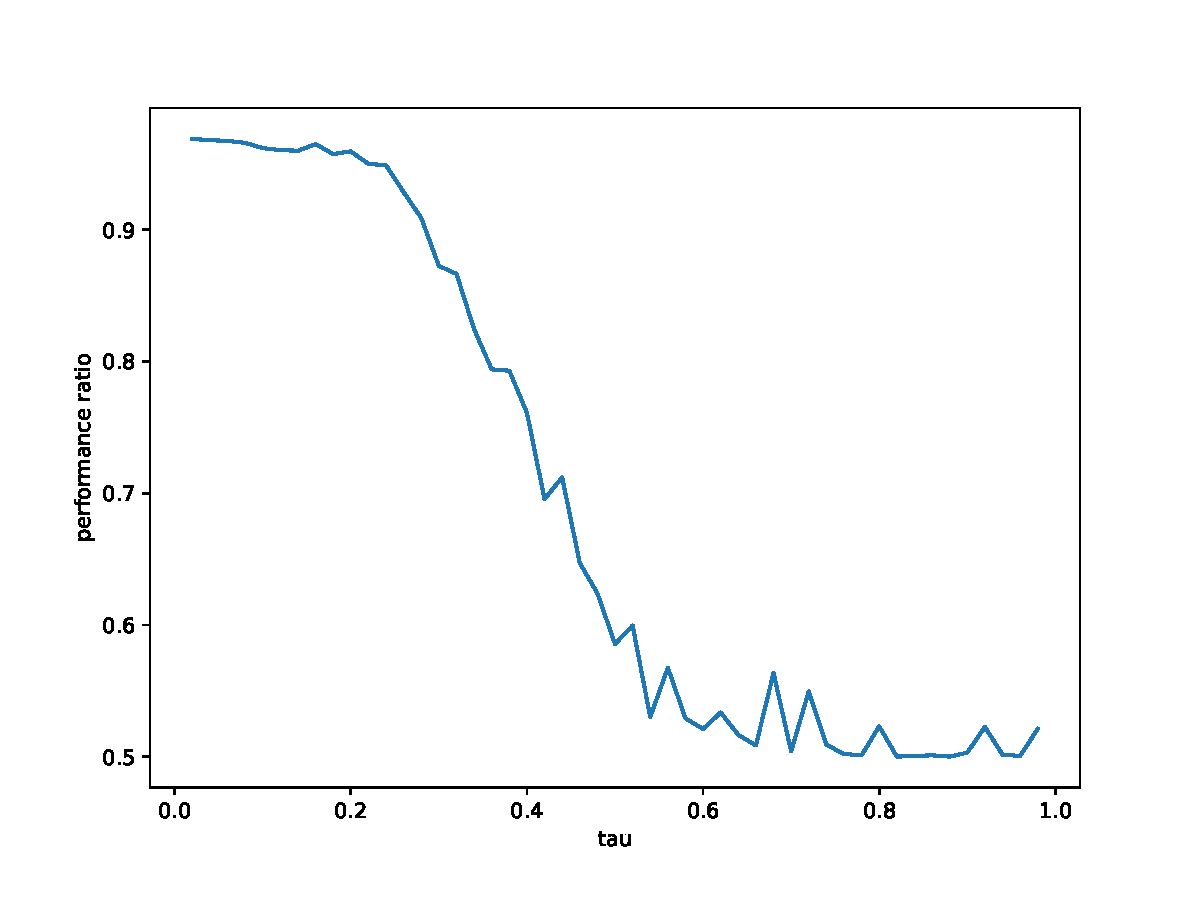
\includegraphics[width=0.8\textwidth]{iris_tau.pdf}
    \caption{Performance of the classifier as a function of $\tau$,
      obtained via the procedure described above}\label{fig:iris-tau}
  \end{figure}

  I've also generated data in $\mathbb{R}^2$ using a mixture of
  gaussian, the result of the decision boundary produced by the SVM
  classifier on these data is shown in the figure \ref{fig:gmm-tau}.
  In both cases, we see that $\tau$ has a significant impact on the
  performance of the classifier (in term of classification error),
  this is expected, because setting a high value of $\tau$ gives more
  importance to the regularity term $\dfrac{1}{2}\norm{w}^2$ and less
  to $\frac{1}{N}\sum_{i = 1}^Nz_i$ in the primal problem, and this is
  the most important term for the classifier to perform well.

  \begin{figure}[h]
    \centering
    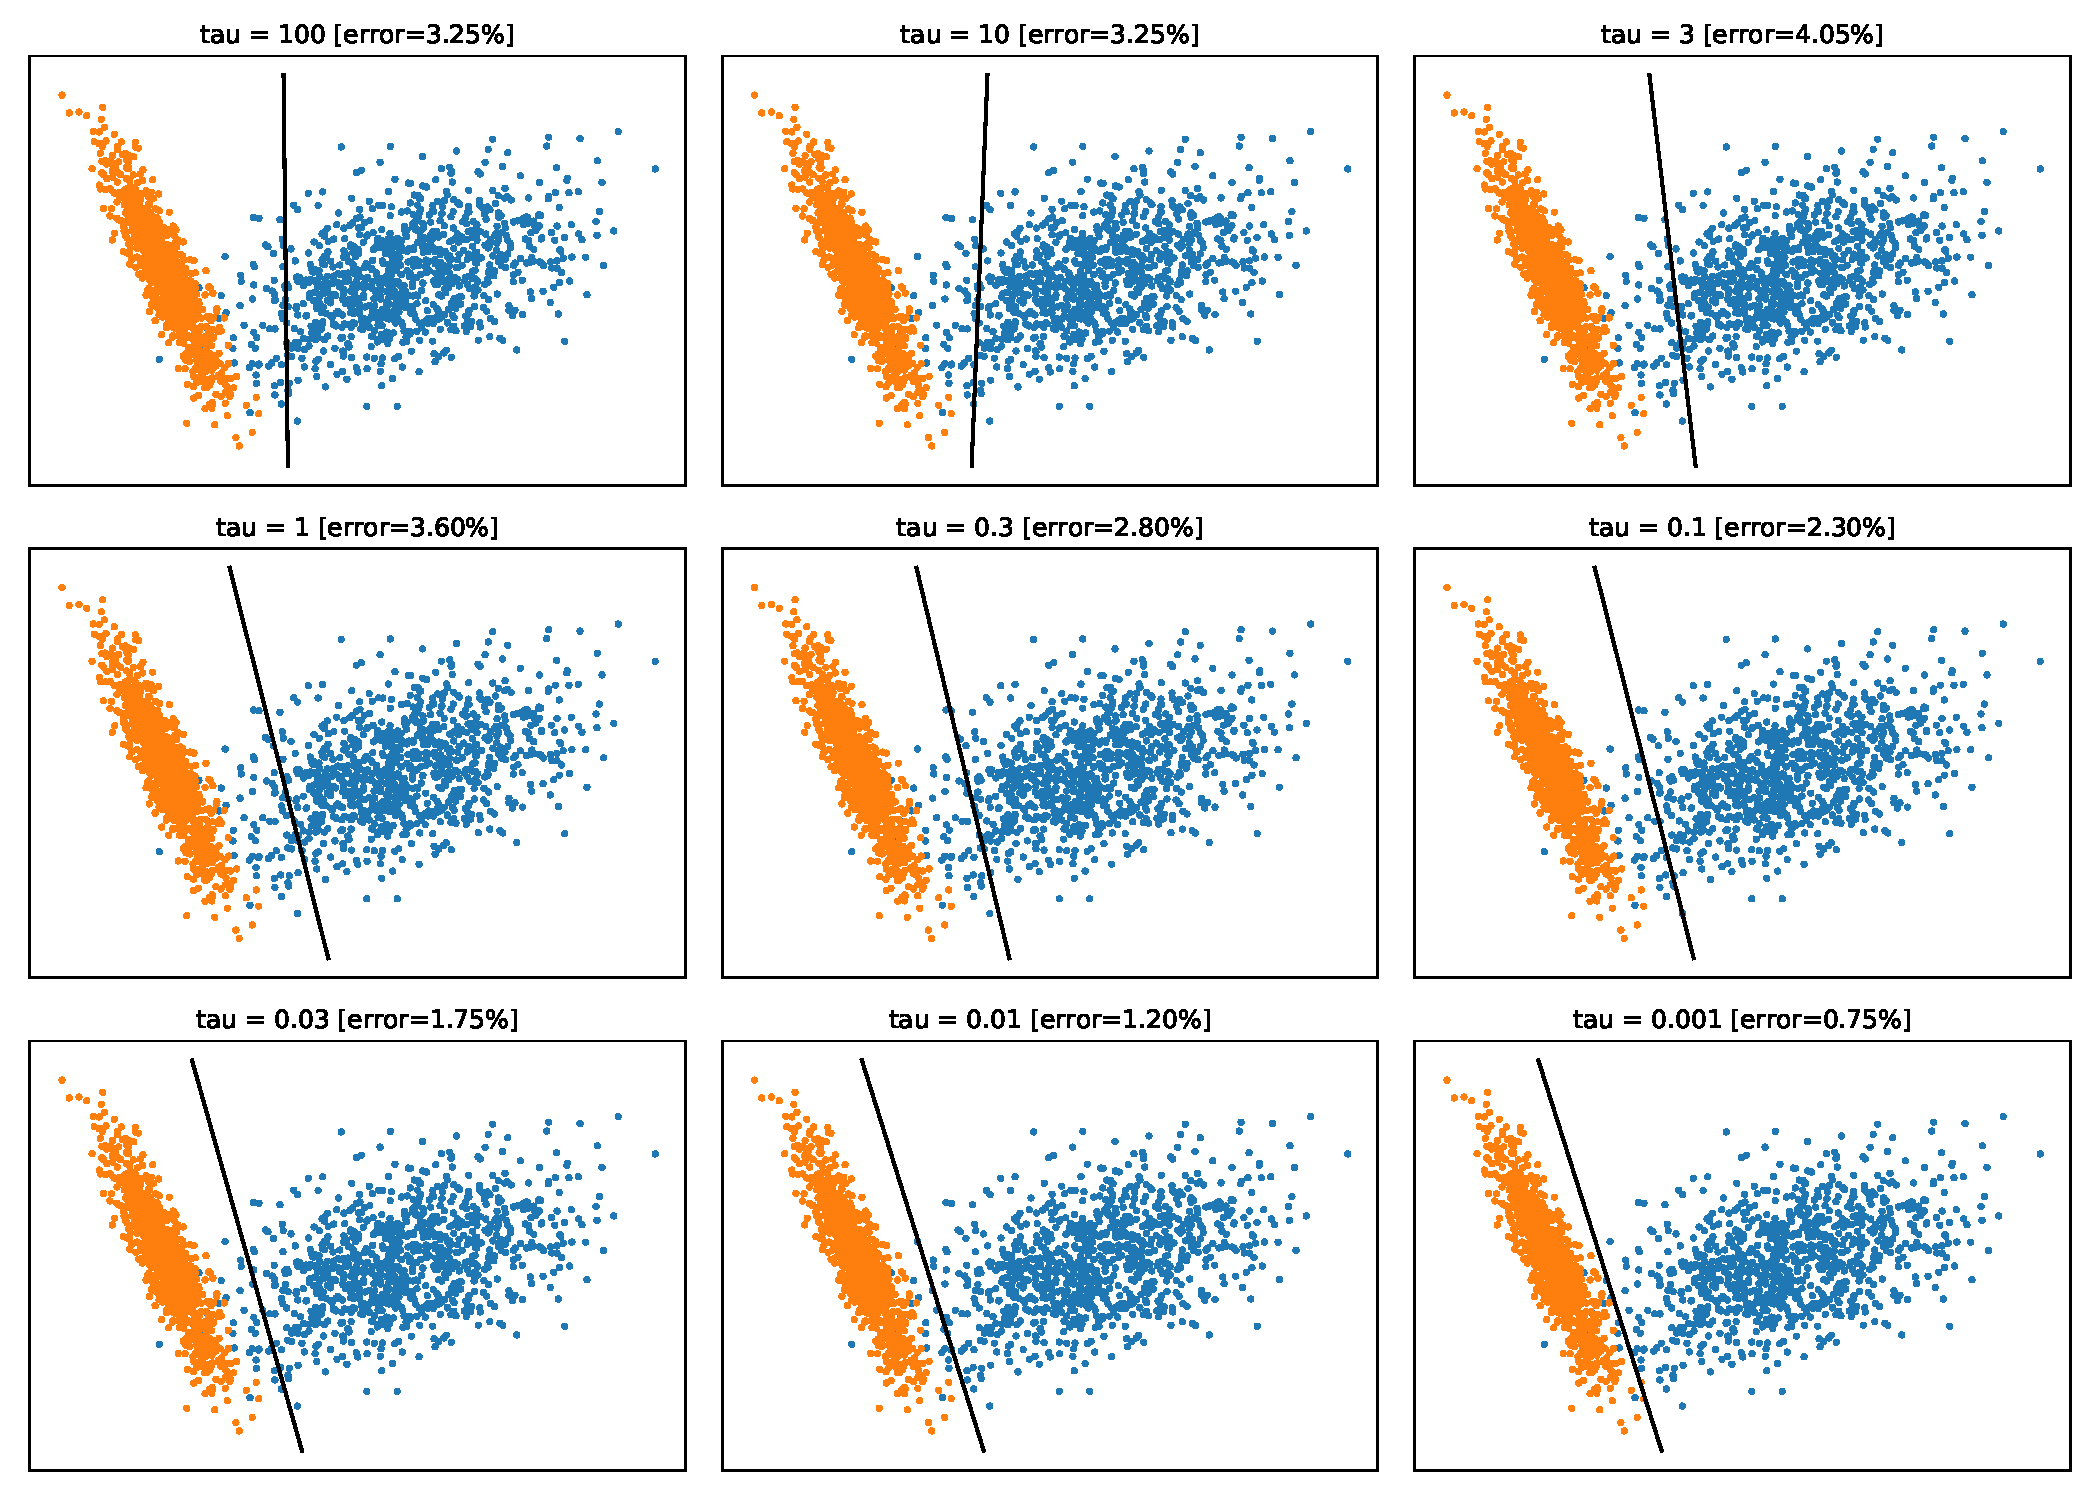
\includegraphics[width=1\textwidth]{gmm_tau.pdf}
    \caption{Representation of the boundary produced by the SVM
      classifier on a gaussian mixture for different values of $\tau$,
      classifier trained on $400$ points ($200$ blue, $200$ orange)
      and evaluated for $2000$ points ($1000$ blue, $1000$
      orange), $\mu = 10$, $tol=10^{-3}$}\label{fig:gmm-tau}
  \end{figure}

\end{question}

\newpage
\begin{question}
  The duality gaps for the primal and the dual problem, for different
  values of $\mu$ are represented in the figure
  \ref{fig:duality-gaps}.

  The figure shows that the number of barrier steps, decreases as
  $\mu$ increases. This is of course not free, since we are
  multiplying $t$ by a higher value at each iteration of the barrier,
  the log barrier is relaxed and the Newton method called at each
  iteration is searching in a much larger space, which requires more
  Newton iterations. We are effectively delegating the complexity to
  the inner Newton calls.

  The table \ref{tab:iteration-mu} presents the total number of step
  needed to solve the primal and the dual SVM problems on the Iris
  dataset for the Damped Newton method and the Newton method with line
  search and a tolerance $\epsilon = 10^{-5}$ and $\tau = 0.01$.
  We see that the total number of Newton iteration does not decrease
  as fast as the number of barrier steps, which confirms the previous
  analysis.

  We can also notice that the Newton method with backtracking line
  search requires less iteration to converge compared to the Damped
  Newton method in our case.  Since Newton steps of both method have
  roughly the same costs (the complexity added by the backtracking
  part can be resumed to computing the function at several points,
  which in our case can be done in $O(n^2)$. This cost is negligeable
  when compared to solving $\nabla^2f(x) \Delta x = \nabla f(x)$ (even
  if it could potentially be multiplied by a high number of
  backtracking iteration, in practice, this is never the case)). Hence
  the Newton Method with backtracking search is performing faster than
  the Damped Newton when training a SVM classifier on the Iris dataset.

  % (We could probably
  % reduce the cost of solving the linear system by exploiting the fact
  % that the matrices are very structured)

  \begin{table}[h!]
    \centering
    \begin{tabular}{|l|c|c|c|c|}
      \hline
      & $\mu = 2$ & $\mu = 15$ & $\mu = 50$ & $\mu = 100$ \\
      \hline
      Damped Newton (Primal) & 323 & 270 & 275 & 273 \\
      Damped Newton (Dual)   & 281 & 224 & 231 & 228 \\
      \hline
      Newton Line search (Primal) & 165 & 60 & 57 & 69 \\
      Newton Line search (Dual)   & 158 & 62 & 53 & 57 \\
      \hline
    \end{tabular}
    \captionof{table}{Total number of iterations needed to train the
      SVM classifier on the Iris dataset, $tol=10^{-5}$,
      $\tau = 0.01$} \label{tab:iteration-mu}
  \end{table}


  \begin{figure}[h]
    \centering
    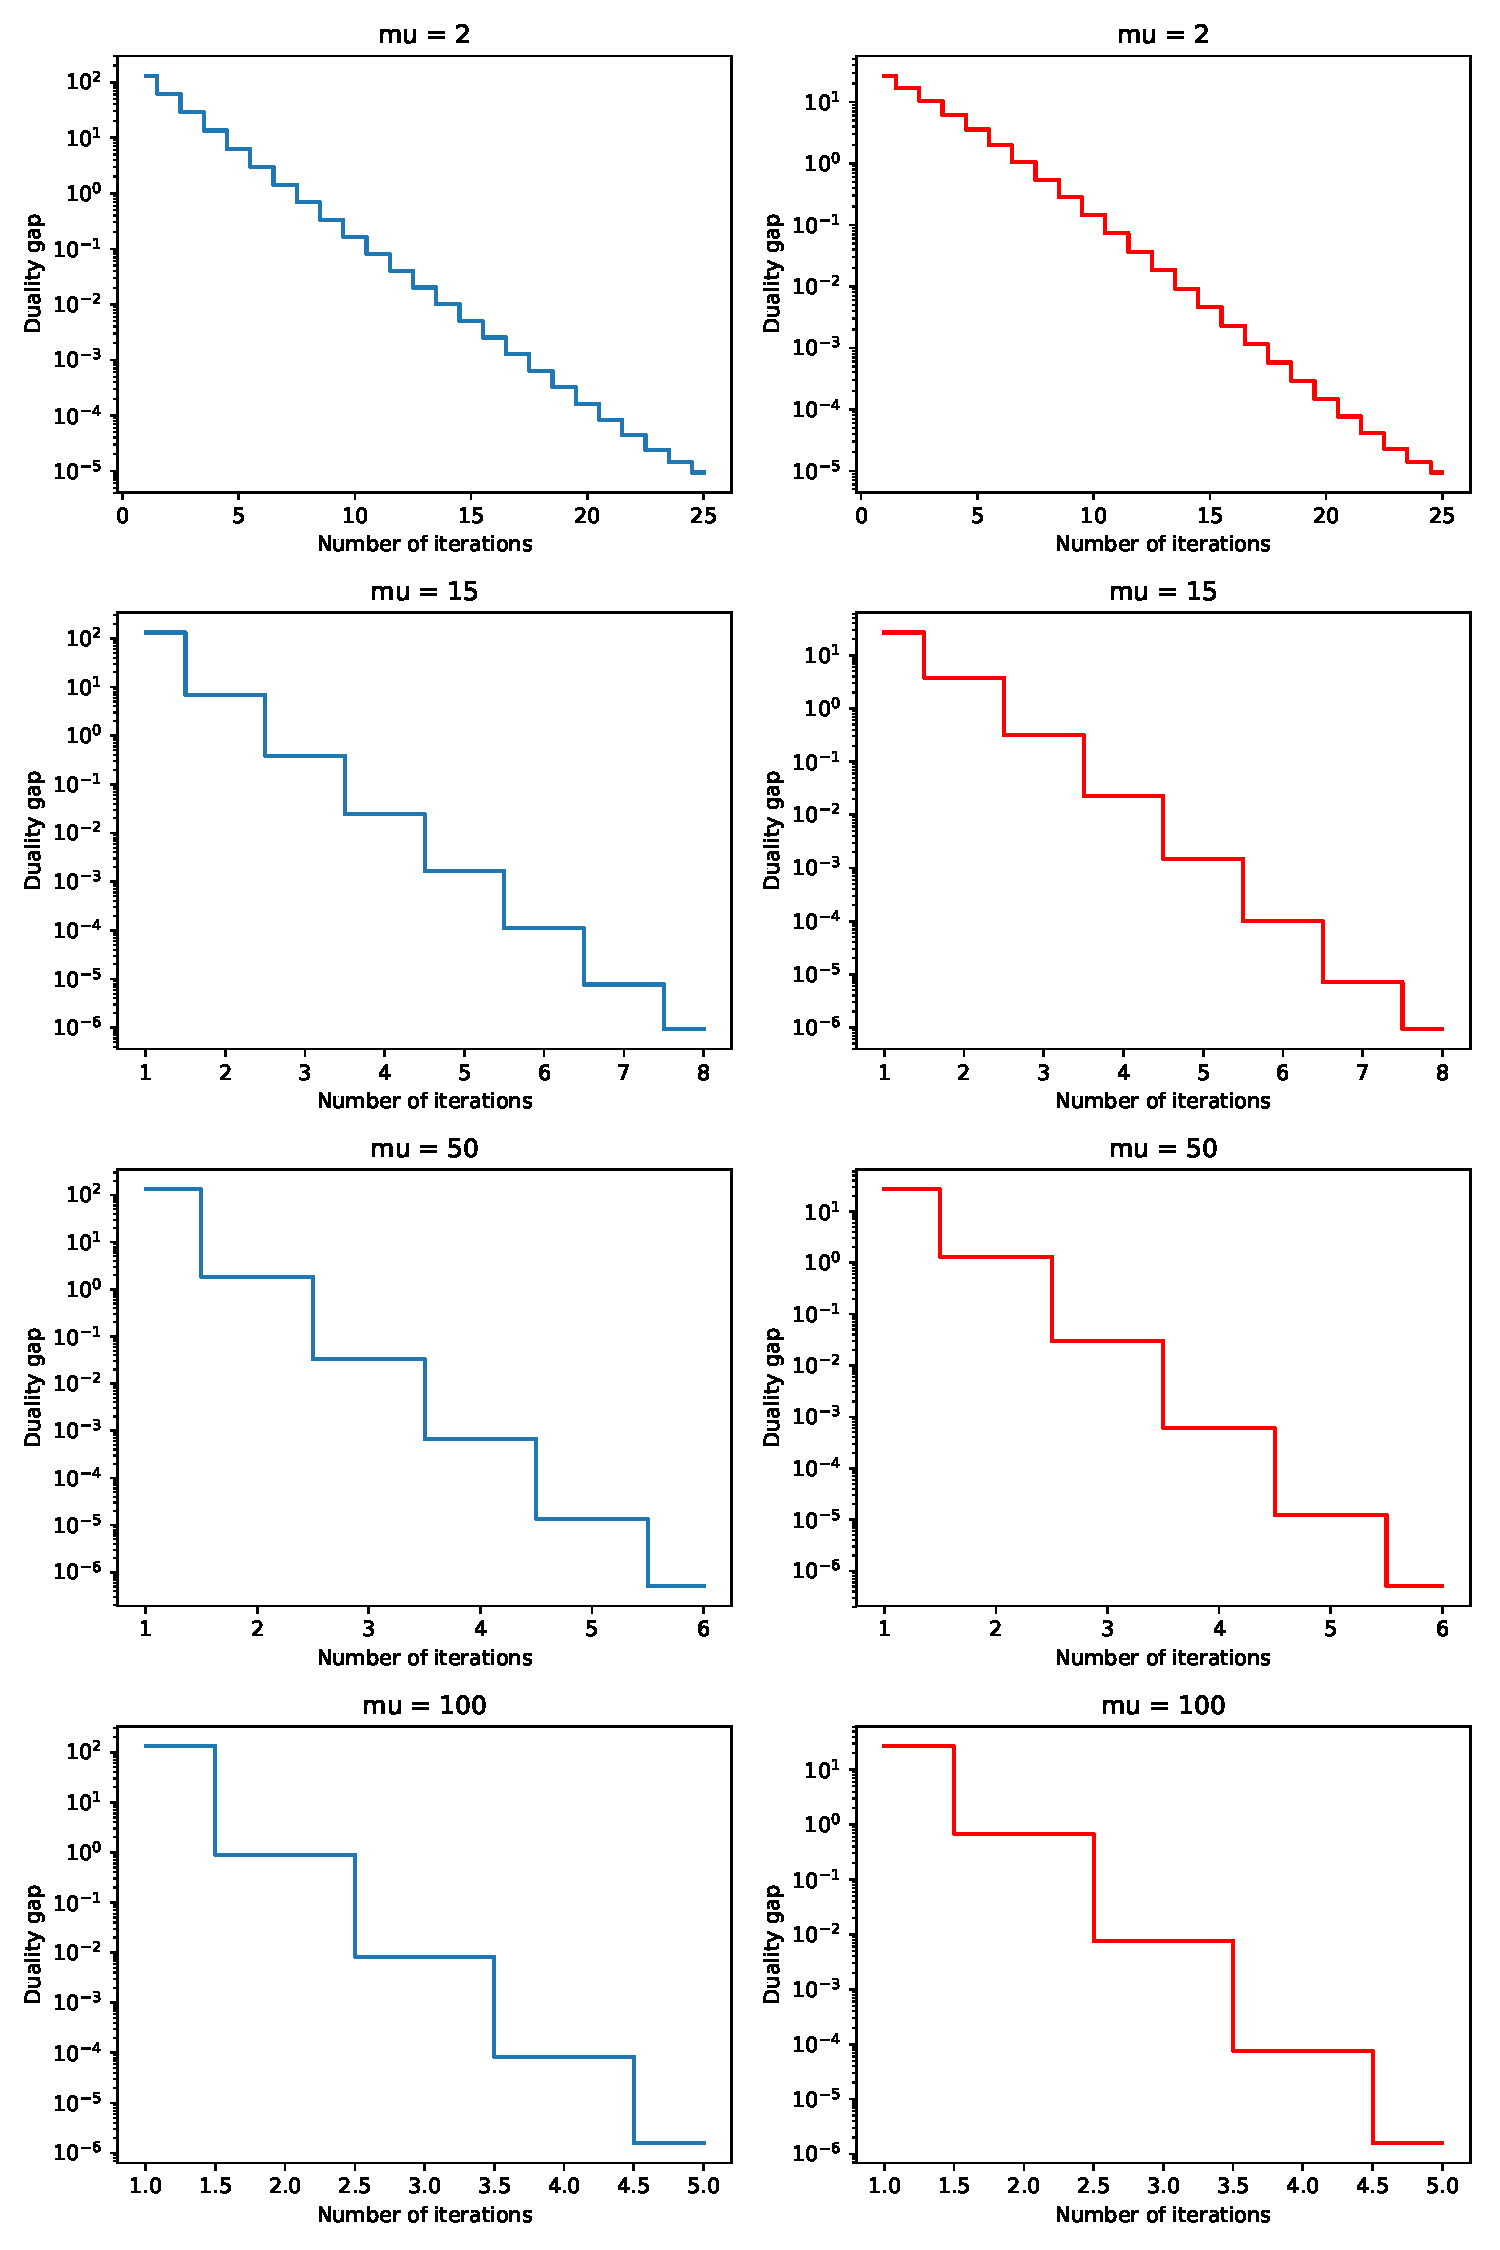
\includegraphics[width=0.80\textwidth]{duality_gaps.pdf}
    \caption{Representation of the duality gap of the primal and the
      dual problem (in semilog scale) for different values of $\mu$
      ($2$, $15$, $50$, $100$), $\epsilon = 10^{-5}$
      $\tau = 0.1$}\label{fig:duality-gaps}
  \end{figure}

\end{question}


  % \begin{table}[h!]
  %   \centering
  %   \begin{tabular}{|c|c|c|}
  %     \hline
  %     & a0 & a1 \\
  %     \hline
  %     s0 & \begin{tabular}{c}
  %            $\pcond{s0}{s0, a0} = 0.45$ \\
  %            $\pcond{s2}{s0, a0} = 0.55$
  %          \end{tabular}
  %     & $\pcond{s2}{s0, a1} = 1.00$ \\
  %     \hline
  %     s1 & $\pcond{s2}{s1, a0} = 1.00$
  %          & \begin{tabular}{l}
  %              $\pcond{s0}{s1, a1} = 0.5$ \\
  %              $\pcond{s1}{s1, a1} = 0.4$ \\
  %              $\pcond{s2}{s1, a1} = 0.1$ \\
  %            \end{tabular}
  %     \\
  %     \hline
  %     s2 & \begin{tabular}{l}
  %            $\pcond{s0}{s2, a0} = 0.6$ \\
  %            $\pcond{s2}{s2, a0} = 0.4$ \\
  %          \end{tabular}
  %     &
  %       \begin{tabular}{l}
  %         $\pcond{s1}{s2, a1} = 0.9$ \\
  %         $\pcond{s2}{s2, a1} = 0.1$ \\
  %       \end{tabular}
  %     \\
  %     \hline
  %   \end{tabular}
  %   \captionof{table}{Representation of the transition table corresponding to the graph
  %     start for $K=4$ } \label{tab:table}
  % \end{table}



%% \begin{figure}[p]
%%   \centering
%%   \begin{subfigure}[t]{0.40\textwidth}
%%     \centering
%%     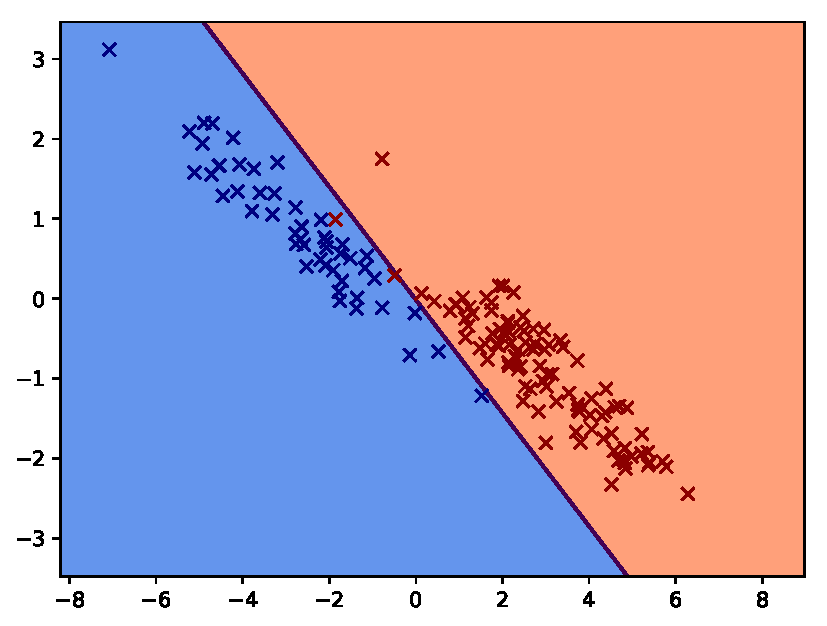
\includegraphics[width=\textwidth]{LDA_classificationA_train.pdf}
%%     \caption{Training observations A ($150$ points)}\label{fig:LDA-A-train}
%%   \end{subfigure}
%%   \quad
%%   \begin{subfigure}[t]{0.40\textwidth}
%%     \centering
%%     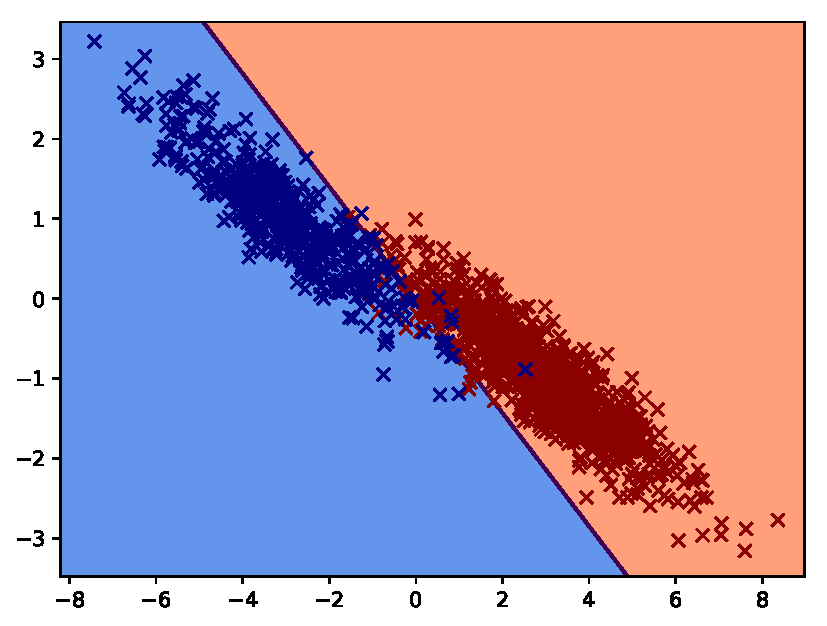
\includegraphics[width=\textwidth]{LDA_classificationA_test.pdf}
%%     \caption{Test observations A ($1500$ points)}\label{fig:LDA-A-test}
%%   \end{subfigure}
%%   \vskip\baselineskip
%%   \begin{subfigure}[t]{0.40\textwidth}
%%     \centering
%%     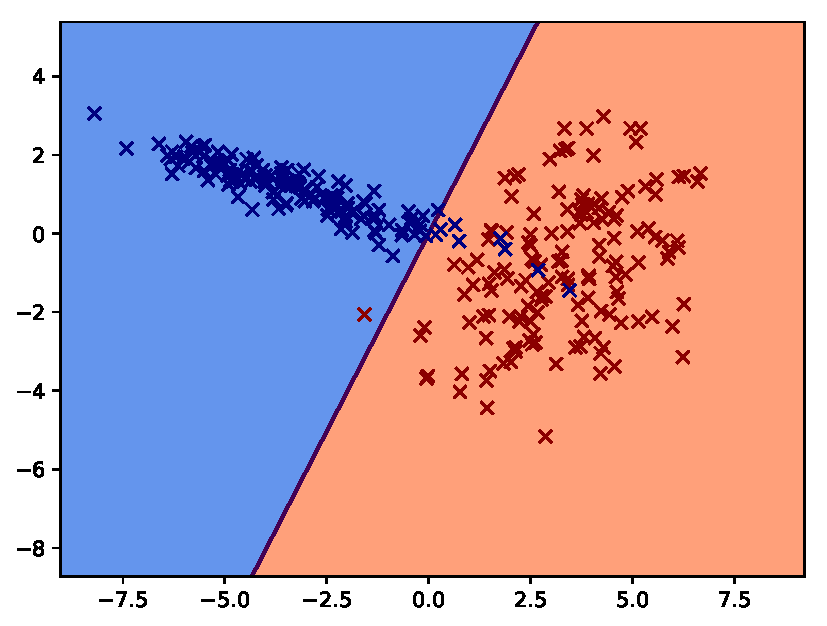
\includegraphics[width=\textwidth]{LDA_classificationB_train.pdf}
%%     \caption{Training observations B ($150$ points)}\label{fig:LDA-B-train}
%%   \end{subfigure}
%%   \quad
%%   \begin{subfigure}[t]{0.40\textwidth}
%%     \centering
%%     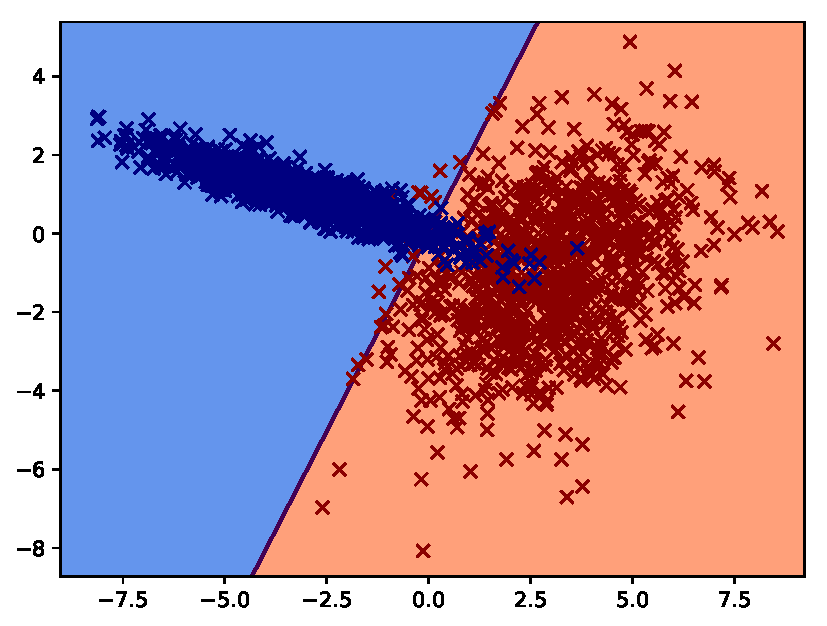
\includegraphics[width=\textwidth]{LDA_classificationB_test.pdf}
%%     \caption{Test observations B ($1500$ points)}\label{fig:LDA-B-test}
%%   \end{subfigure}
%%   \vskip\baselineskip
%%   \begin{subfigure}[t]{0.40\textwidth}
%%     \centering
%%     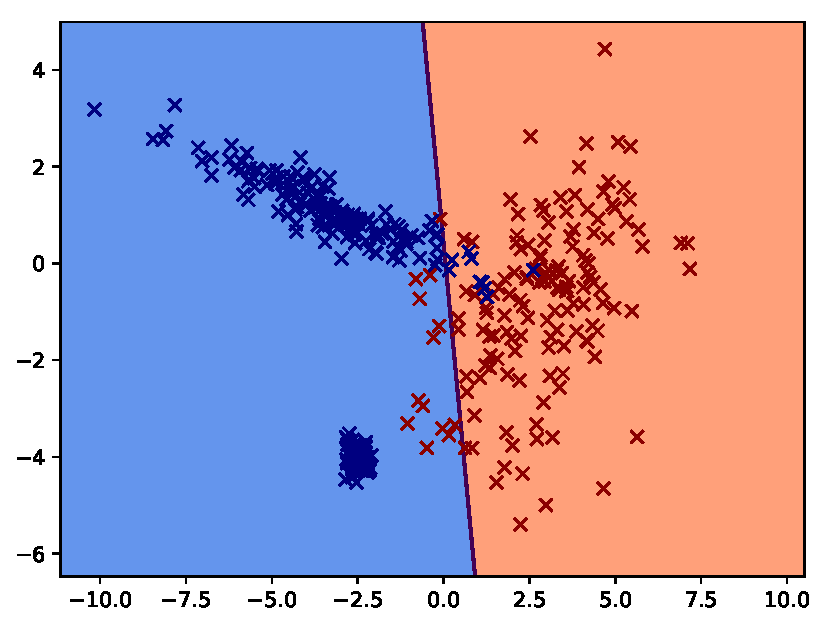
\includegraphics[width=\textwidth]{LDA_classificationC_train.pdf}
%%     \caption{Training observations C ($150$ points)}\label{fig:LDA-C-train}
%%   \end{subfigure}
%%   \quad
%%   \begin{subfigure}[t]{0.40\textwidth}
%%     \centering
%%     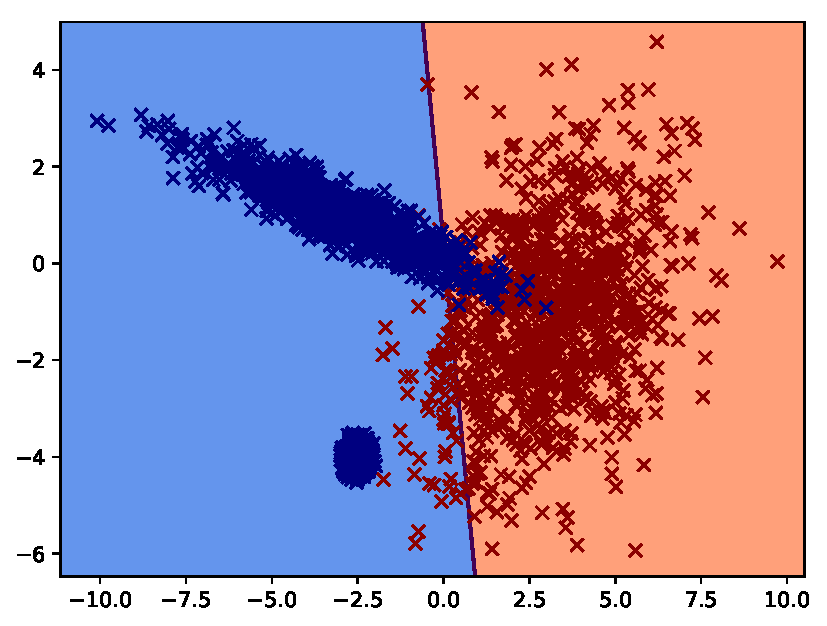
\includegraphics[width=\textwidth]{LDA_classificationC_test.pdf}
%%     \caption{Test observations C ($1500$ points)}\label{fig:LDA-C-test}
%%   \end{subfigure}
%%   \caption{Sample data and decision boundary representation for the LDA classifier on the three files}\label{fig:LDA}
%% \end{figure}


\end{document}
